\section{Introduction}

\key{Recommender Systems}{Information Retrieval}{Supervised Learning}{Unsupervised Learning}{Regression}{Classification}{Clustering}{Projection}

\lecture{30}{10}{2020}

\par{ML starts with data, and the two key questions/problems are if we can find similarities across the different observations and if we can make predictions about them. Nowadays, ML can be though of as an ever-growing set of algorithms, which can be hard to understand and use and which may have to be tuned. Hence, it is important to understand them}

\par{AI move in the 70s evolves towards NN which can be seen as a function. During that time some studies shown that those functions did quite well at approximating certain kinds of behaviours, and so they tried to scale up to more complex tasks. They quickly realise that the real world was far too complex to be modelled in this manner, and so researchers focused on 2 key aspects : modelling the brain and predictions from data}


\subsection{Course Topics}

	\begin{itemize}
		\item Learning from data
		\item Caveats
		\item Examining common algorithms
		\item How to implement algos and use popular libraries
		\item Essential maths and stats
	\end{itemize}

\subsection{Prerequisites}
	\par{only the fundamentals, nothing too advanced}

	\begin{itemize}
		\item Linear Algebra 
		\item Probability and Random Variables
		\item Calculus
		\item Logs
		\item Python (scientific stack)
	\end{itemize}



\subsection{Real World Applications}

	\par{Recommender Systems are one of the most popular applications in ML, specifically because it is hard to use a physical model to describe one's preferences, i.e you can't really write a traditional equation which describes preferences. However, given enough data, we can look for patterns}

	\par{Biotech companies are others who make use of ML in order to diagnose patients and discover \ita{biomarkers}. The patients can then be clustered into groups which improves the efficacy of clinical trials.}


	\par{Within the SoCS the IR group use ML for such tasks as search, topic identification in noisy environments (e.g. news feeds), language models and video annotation. Within the HCI group ML is applied to improve speech and gesture recognition}


\subsection{Supervised and Unsupervised Learning}

	\subsubsection{Supervised}

		\defn{Regression}{a type of model that outputs continuous values}

		\par{Regression, is essentially using a continuous function to learn from a set of examples. The algorithm learns by trying to fit the data to the regression line}

		\example{predicting stock prices where $x$ is time}

		\defn{Classification}{model for distinguishing among two or more discrete classes}

		\par{Classification, learning a rule that can separate objects of different types from another. In this case, the output variable $y$ is no longer continuous, we want $f(x)$ to group its inputs and spit out a \ita{discrete} choice (e.g [1,0]). So we can see it as providing a decision boundary between elements of different groups}

		\example{Predicting skin cancer: we take images of moles filter them trough our $f(x)$ which will classify them as either malignant or benign}

	\subsubsection{Unsupervised}

		\defn{Clustering}{}

		\par{We'll focus on the problem of clustering, i.e trying to find subgroups in the measures that we have. The key difference being that the data is not labelled}

		\example{people with similar tastes, genes with similar functions}

		\defn{Projection}{}

		\par{Projection, when we have data with a lot of dimensions which can be hard to visualise. We can use projection to reduce the number of related variables without losing the essential meaning/info.}

		\example{Genetics (PCA), where the original data is a binary matrix where each column is a \ita{snip} and each row represents a person }


\section{Supervised Learning - Linear Modelling}

\lecture{30}{09}{20}

	$\begin{array}{l}\text { Linear models } \\ \text { - Introduce the idea of building models. } \\ \text { - Talk about assumptions. } \\ \text { - Use a linear model. } \\ \text { - What constitutes a good model? } \\ \text { - Find the best linear model. } \\ \text { - Use it to predict the winning time in 2012. }\end{array}\\$

	\par{In this lecture we'll use the dataset provided in section 1.1 of the textbook. Our goal will be to formalise this fitting and prediction process via a mathematical model which will allow us to scale this method to bigger problems}



	\subsection{Building Models}

	\IfFileExists{assets/olympics.png}{}{\immediate\write18{wget https://cdn.mathpix.com/snip/images/R_QTQtLEy01fTnHSGS9KxPRaiP7Q70amUHROp5ZSetM.original.fullsize.png -O assets/olympics.png}}
	\begin{figure}[ht]
	\centering
	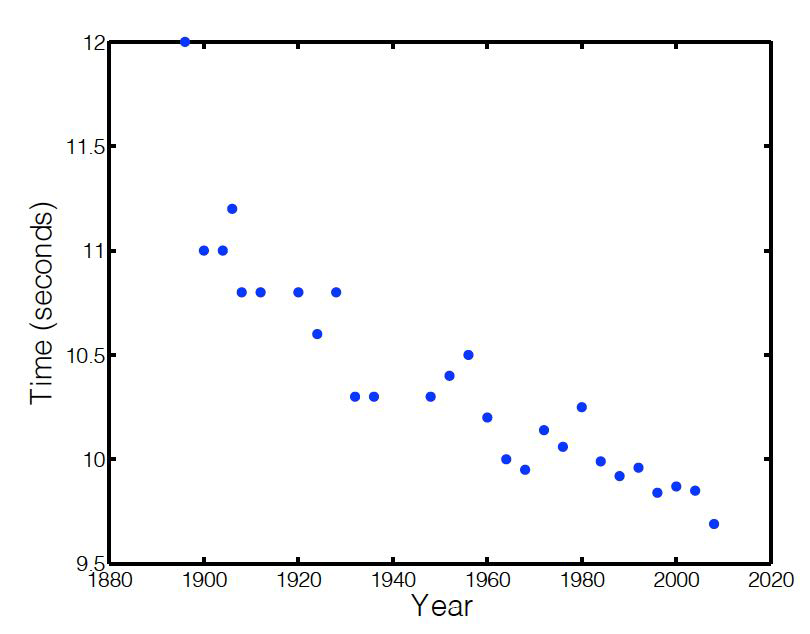
\includegraphics[width=0.5\textwidth]{assets/olympics.png}
	\end{figure}


		\subsubsection{Formalizing Intuitions}


	\begin{minipage}{\linewidth}
	      \centering
	      \begin{minipage}{0.45\linewidth}
	          \begin{itemize}
	          	\item Decided to draw a line through our data
	          	\item Chose a straight line
	          	\item Drew a good straight line
	          	\item Extended the line to 2012
	          	\item Read off the winning time for 2012
	          \end{itemize}
	      \end{minipage}
	      \hspace{0.05\linewidth}
	\begin{minipage}{0.45\linewidth}
	          \begin{itemize}
	          	\item Decided we need a model
	          	\item Chose a linear model
	          	\item Fitted a linear model
	          	\item Evaluated the model at 2012
	          	\item Used this as our prediction
	          \end{itemize}
	      \end{minipage}
	\end{minipage}


		\subsubsection{Assumptions}

		\par{When approaching the problem, we decided to assume the following:}

			\begin{enumerate}
				\item there exists a meaningful relationship between year and winning time
				\item the relationship is linear
				\item the relationship will continue into the future
			\end{enumerate}

		\par{We are now going to investigate if we were right to do so}



	\subsection{Mathematically Defining the Model}


		\defn{Attributes/Features}{an input variable used in making predictions}

		\example{Olympic year}

		\defn{Targets/Labels}{in supervised learning, the answer portion of the example (e.g. spam/not spam)}

		\example{Winning time}

		\defn{Model}{the representation of what a machine learning system has learned from the training data, i.e some function which maps inputs to outputs}

		\example{$f(x) = t$}

		\defn{Training Data}{the subset of the dataset used to train a model}

		attribute-response pairs


		\defn{Linear Model}{ a model that assigns one weight per feature to make predictions

		$$t = f(x) = w_o + w_1x = f(x ; w_0,w_1)$$
		}

		\par{Our linear model is essentially a line which can be \ita{parametrized}. Usually a weight for bias is also included. In this example we only have our features represented by $x$ and the feature's weights/parameters $w$ which determine the properties of the line.}

		\rem{note that this is simple high school geometry, you're tweaking the slope and $y$-intercept}

		\subsubsection{Loss Function - Finding the right W}

			\par{Now that we have data and a \ita{family} of models we need to find the best $(w_o, w_1)$ pair so that our model fits our data as best as possible. We are going to find the pair from the set of $(x_1,t_1), \dots, (x_n,t_n)$ training examples}

			\par{In order to do this we compare each pair given by our model against the expected value, and our goal here is to minimise the error. So we sum over all the pairs to find out the total cost of that particular model and we pick the parameters $w$ which give us the smallest total cost}


			\defn{Loss/Cost Function}{a function used for parameter estimation that maps an event like our (expected - estimated) function to a real number}

			\IfFileExists{assets/loss1}{}{\immediate\write18{wget https://cdn.mathpix.com/snip/images/fuITHo1Hde0D4wyjlh3gSEUFnVBzBiJISBe9McB4hdQ.original.fullsize.png -O assets/loss1}}
			\IfFileExists{assets/loss2}{}{\immediate\write18{wget https://cdn.mathpix.com/snip/images/BOfyRGM1XhT1qxUUDi5rHdc1jGcpn5C6ytwh3XXwiBM.original.fullsize.png -O assets/loss2}}

			\begin{minipage}{\linewidth}
			\centering
			\begin{minipage}{0.45\linewidth}
			\begin{figure}[ht]
			\includegraphics[width=0.5\textwidth]{assets/loss1}
			\end{figure}
			\end{minipage}
			\hspace{0.05\linewidth}
			\begin{minipage}{0.45\linewidth}
			\begin{figure}[ht]
			\includegraphics[width=0.5\textwidth]{assets/loss2}
			\end{figure}
			\end{minipage}
			\end{minipage}

			\defn{Squared Loss}{The average squared loss per example, which is calculated by diving the squared loss by the number of examples}

			$$\mathcal{L}_{n}=\left(t_{n}-f\left(x_{n} ; w_{0} ; w_{1}\right)\right)^{2}$$

			\rem{we need to square the mean to get the absolute values of each loss}

			\par{By taking the mean, we can now have a loss function which tells us something about how the model did \ita{on average}.}

			$$\mathcal{L}=\frac{1}{N} \sum_{n=1}^{N}\left(t_{n}-f\left(x_{n} ; w_{0}, w_{1}\right)\right)^{2}$$

			
















